% Select language used in document (ngerman or english). Automatically
% generated text is translated accordingly.
% use \selectthesislanguage in body.tex to switch to default language

\documentclass[english, paper]{mmt} % use for BA1
%\documentclass[english, bachelorthesis]{mmt} % use for BA2
%\documentclass[ngerman, masterthesis]{mmt} % use for Master thesis

\usepackage{mathptmx}
\usepackage{graphicx}
\usepackage{times}
\usepackage{subfig}
\usepackage{float}
\usepackage[utf8]{inputenc}
\usepackage{listings}
\usepackage{makecell}
\usepackage[anythingbreaks]{breakurl}

\usepackage{amsmath}
\usepackage[autostyle,german=guillemets]{csquotes}

% moved to cls file. use \selectthesislanguage to switch to default language
%\usepackage[english,ngerman]{babel}

\usepackage{abbrevs}
%% the following solves a bug in the abbrevs package, that adds an empty
%% space after the abbrev
\makeatletter
\renewcommand\maybe@space@{%
  % \@tempswatrue % <= this is in the original
  \maybe@ictrue % <= this is new
  \expandafter   \@tfor
    \expandafter \reserved@a
    \expandafter :%
    \expandafter =%
                 \nospacelist
                 \do \t@st@ic
  % \if@tempswa % <= this is in the original
  \ifmaybe@ic % <= this is new
    \space
  \fi
}
\makeatother
%%


\usepackage{listings}
\usepackage{color}
\definecolor{lightgray}{rgb}{.9,.9,.9}
\definecolor{darkgray}{rgb}{.4,.4,.4}
\definecolor{purple}{rgb}{0.65, 0.12, 0.82}
\lstdefinelanguage{JavaScript}{
  keywords={break, case, catch, continue, debugger, default, delete, do, else, false, finally, for, function, if, in, instanceof, new, null, return, switch, this, throw, true, try, typeof, var, let, const, void, while, with},
  morecomment=[l]{//},
  morecomment=[s]{/*}{*/},
  morestring=[b]',
  morestring=[b]",
  ndkeywords={class, export, boolean, throw, implements, import, this},
  keywordstyle=\color{blue}\bfseries,
  ndkeywordstyle=\color{darkgray}\bfseries,
  identifierstyle=\color{black},
  commentstyle=\color{purple}\ttfamily,
  stringstyle=\color{red}\ttfamily,
  sensitive=true
}

\lstset{
   language=JavaScript,
   backgroundcolor=\color{lightgray},
   extendedchars=true,
   basicstyle=\footnotesize\ttfamily,
   showstringspaces=false,
   showspaces=false,
   numbers=left,
   numberstyle=\footnotesize,
   numbersep=9pt,
   tabsize=2,
   breaklines=true,
   showtabs=false,
   captionpos=b
}

\usepackage[authordate,bibencoding=auto,strict,noibid,backend=biber]{biblatex-chicago}
\bibliography{bibliography}

%% Add configuration options
\newabbrev{\authorname}{Isabella Margarita Sperr}
\newabbrev{\authormail}{isperr.mmt-b2016@fh-salzburg.ac.at}
\newabbrev{\titlename}{Using eye tracking to improve web UX}
\newabbrev{\advisor}{DI Michael Domhardt}
%\newabbrev{\secondadvisor}{Titel Vorname Nachname}
\newabbrev{\thesisdate}{22.05.2018}
\newabbrev{\keywordsenglish}{word1, word2, word3}
\newabbrev{\keywordsgerman}{wort1, wort2, wort3}


%% Paper title.

\title{\titlename}

%% This is how authors are specified in the conference style

%% Author 
\author{ \authorname\\ \scriptsize \authormail \\ \scriptsize 
\ifmmtlanguagegerman FH Salzburg \else Salzburg University of Applied Sciences \fi
}

%% A teaser figure can be included as follows, but is not recommended since
%% the space is now taken up by a full width abstract.
%\teaser{
%  \includegraphics[width=1.5in]{sample.eps}
%  \caption{This can be a teaser image of the thesis.}
%}

%% Abstract section for paper format.
\abstract{
    \ifmmtlanguagegerman 
        \selectlanguage{ngerman}
        Diese Bachelorarbeit bietet einen Einblick in das Beobachtungsverhalten eines Webbenutzers, wenn dieser im Internet eine Suchmaschine benutzt. Um besser zu verstehen, wie verschiedene User eine Suchergebnisseite (search engine result page -- SERP) einer üblichen Suchmaschine betrachten und verwenden, kann ein Eye Tracking Gerät angebracht werden. Dieses zeichnet die Augenbewegungen eines Benutzers auf, damit die Daten zu einem späteren Zeitpunkt ausgewertet werden können \autocite{liu2015influence}. Daher ist es notwendig, die relevantesten Eye Tracking Technologien, Parameter und Visualisierungsmethoden näher zu betrachten. Darüber hinaus konzentriert sich diese Arbeit auf Suchergebnisseiten, wie sie aufgebaut sind und wie der Benutzer die dort präsentierten Informationen erfasst und verarbeitet.
Um besser zu verstehen wie SERPs aufgebaut sind, wie die Ergebnisseite näher an einem Beispiel einer modernen kommerziellen Suchmaschine erklärt.
Darüber hinaus gibt es einen Vergleich moderner Suchmaschinen, der die Vorteile und Nachteile der SERP-Struktur betont.
Nur wenn diese Anforderungen erfüllt werden, kann eine Suchergebnisseite verbessert und entsprechend angepasst werden, um die Effizienz der Informationsgewinnung zu maximieren.

    \else 
        \selectlanguage{english}
        ... will follow shortly ...
    \fi
}


%%%%%%%%%%%%%%%%%%%%%%%%%%%%%%%%%%%%%%%%%%%%%%%%%%%%%%%%%%%%%%%%
%%%%%%%%%%%%%%%%%%%%%% START OF THE PAPER %%%%%%%%%%%%%%%%%%%%%%
%%%%%%%%%%%%%%%%%%%%%%%%%%%%%%%%%%%%%%%%%%%%%%%%%%%%%%%%%%%%%%%%%

\begin{document}

\selectthesislanguage

\pagenumbering{gobble}

 % group open
\ifmmtpaper 
\begingroup 
    % is required because paper template messes with sizes
    \fontsize{12}{18}\selectfont        
    \setlength{\parindent}{0pt}
    \setlength{\parskip}{5pt plus 2pt minus 1pt}
    \sectionfont{\fontsize{14}{15}\selectfont}
\fi

    \begin{titlepage}

% check if second advisor exists
\newcommand{\printsecondadvisor}[1]{%
  \ifcsname#1\endcsname%
  \ifmmtlanguagegerman ZweitbetreuerIn: \else Second Advisor: \fi \secondadvisor 
  \else%
    
  \fi%
}

\ifmmtmasterthesis

    
    % \begin{center}
    %     \Huge{ 
    %     	\textbf{\ifmmtlanguagegerman Masterarbeit \else Master Thesis \fi}
    %     }
    % \end{center}
    
    \newpage
    
    \thispagestyle{empty}
    
    \hfill 
\includegraphics[height=1.5cm]{images/FHSLogo.jpg}
    
    \vspace*{2cm}
    
    \Large{
    \titlename
    
    \vspace*{1cm}
    
    \ifmmtlanguagegerman
    Masterarbeit zur Erlangung des akademischen Grades
    \else
    Master thesis in partial fulfilment of the requirements for\\ the degree of 
    \fi
    
    \vspace*{0.5cm}
    
    \textit{Master of Science}
    }
    
    
    \vspace*{1.5cm}
    {\large
    \ifmmtlanguagegerman AutorIn \else Author \fi: \authorname
    }
    \vfill
    
    {\normalsize
    \ifmmtlanguagegerman
    Vorgelegt am FH-Masterstudiengang MultiMediaTechnology, Fachhochschule Salzburg
    \else
    Submitted to the Master degree program MultiMediaTechnology, Salzburg University of Applied Sciences
    \fi
    
    
    \vspace*{1cm}
    
    \ifmmtlanguagegerman BetreuerIn: \else Advisor: \fi
    \advisor
    \\    
    \printsecondadvisor{secondadvisor}
    
    \vfill
    
    Salzburg, \ifmmtlanguagegerman Österreich, \else Austria, \fi  \thesisdate
    }

\else % Bachelor thesis title page

    \begin{center}
    
    
\includegraphics[width=5cm]{images/FHSLogo.jpg}


    \vspace*{4cm}
    
    \fontsize{20.79}{18pt}{\selectfont        
    %\Large{
    	\textit{\textbf{\titlename}}
    %}
    }
    
    \vspace*{4cm}
    
    \fontsize{20.79}{18pt}{%\large{
    \ifmmtlanguagegerman
    	\textbf{Bachelorarbeit \ifmmtpaper 1 \else 2 \fi }
    \else
        \textbf{Bachelor Thesis \ifmmtpaper 1 \else 2 \fi }
    \fi
    }
    
    
    \end{center}
    
    \vfill
    
    %\begin{tabular}{ll}
    \ifmmtlanguagegerman AutorIn: \else Author: \fi  \authorname  \\
    \ifmmtlanguagegerman BetreuerIn: \else Advisor: \fi \advisor \\
    \printsecondadvisor{secondadvisor}
    
    Salzburg, \ifmmtlanguagegerman Österreich, \else Austria, \fi \thesisdate
    
    
    
    % uncomment the following 3 lines for an optional lock flag, max. 2 years!
    %\hfill
    %\color{red}
    %\framebox{Sperrvermerk bis 20/01/2012}

\fi

\end{titlepage}
        
    \onecolumn           
    
    \pagenumbering{roman}
    
    \newpage
    
\ifmmtlanguagegerman
\subsection*{Eidesstattliche Erklärung}


Ich erkläre hiermit eidesstattlich, dass  ich  die vorliegende Arbeit selbständig  und ohne fremde Hilfe verfasst, und keine  anderen  als die angegeben Quellen und  Hilfsmittel benutzt  habe. Weiter versichere ich hiermit, dass ich   die den benutzten Quellen  wörtlich oder inhaltlich entnommenen Stellen als solche kenntlich gemacht habe.

Die Arbeit wurde bisher in gleicher oder ähnlicher Form keiner anderen Prüfungskommission weder im In- noch im Ausland vorgelegt und auch nicht veröffentlicht.

\else

\subsection*{Affidavit}

I herewith declare on oath that I wrote the present thesis without the help of third persons and without using any other sources and means listed herein; I further declare that I observed the guidelines for scientific work in the quotation of all unprinted sources, printed literature and phrases and concepts taken either word for word or according to meaning from the Internet and that I referenced all sources accordingly.

This thesis has not been submitted as an exam paper of identical or similar form, either in Austria or abroad and corresponds to the paper graded by the assessors.

\fi

\vspace*{3cm}

%{\bf \thesisdate{}}


\hfill

\ifmmtlanguagegerman
$\overline{Datum \hspace{2cm}}$ \hfill $\overline{{Unterschrift}\hspace{3cm}}$

\vspace*{1cm}

\hfill $\overline{{Vorname\hspace{2cm}Nachname}}$
 
 \else
 $\overline{Date \hspace{2cm}}$ \hfill $\overline{{Signature}\hspace{4cm}}$

\vspace*{1cm}

 \hfill $\overline{{First~Name\hspace{2cm}Last~Name}}$
 \fi

  % comment out for expose

% group closing
\ifmmtpaper
\endgroup
\fi

%\ifmmtpaper\else
    
    \ifmmtmasterthesis    
    \vspace*{0.5cm} 
    \textbf{Schlüsselwörter:~} \keywordsgerman
    \fi
    
    \newpage
    \selectlanguage{english}
    \section*{Abstract}
    ... will follow shortly ...
    
    \ifmmtmasterthesis        
    \vspace*{0.5cm} 
    \textbf{Keywords:~} \keywordsenglish
    \fi
    
    \selectthesislanguage
    
    \newpage
    \tableofcontents

%\fi

\mmtcolumnmode % switch back to column formatting of stylesheet

\maketitle % used for paper formatting

\ifmmtpaper\else
\pagestyle{headings}
\fi
\pagenumbering{arabic}


%for reference to this section
\section{Introduction}
\label{section:Introduction}
... will follow shortly ...

\section{Reading}
\label{section:Reading}

\subsection{Eye}
\label{subsection:Eye}

\subsubsection{Physiological}

\subsubsection{Movements}

\subsection{Information Processing}
\label{subsection:InformationProcessing}

\subsection{Differences between German and English}
\label{subsection:Differences}

\section{Eye Tracking}
\label{section:EyeTracking}
When an eye tracking device is being used, someone's eye movements are being recorded. This recorded material, the raw eye tracking data, can be evaluated and the resulting parameters (e.g., fixation, saccades, regression, etc.) can be summed up in visualization graphs \autocite[]{goldberg2002eye, poole2006eye, beymer2007eye}. Hence, eye tracking can be used as a valuable tool in many web application cases such as creating webpages, placing advertisements or arranging search engine result pages \autocite{buscher2009you, liu2015influence}. \textcite[]{buscher2009you} note in their paper that web developers can also profit from taking eye tracking study results into consideration when designing and styling their new websites. 

However, eye tracking is not only used for webpages. For instance, another outstanding application case is psychology, where the eye tracker is used to record the eye movements while doing any kind of information process, e.g. reading \autocite{schiessl2003eye}.
Accordingly, when it comes to online reading, eye tracking has been a helpful expedient to gain information on how the human brain processes information retrieved from a text \autocite[]{schiessl2003eye}.
As a result, the following section will include the most popular technologies, parameters and accordingly the required visualization methods. 

\subsection{Technologies}
\label{subsection:Technologies}
As \textcite[]{biedert2010eyebook} is expressing in their paper, eye tracking has been around for more than 100 years, and researchers gained a lot of important data. As a consequence, eye tracking technology has evolved a lot over these several years \autocite[]{poole2006eye}.
For example, in the time since the first eye tracking devices have been invented, they have come a long way. In the early beginnings, direct contact with the cornea was necessary as \textcite[]{jacob2003eye} mention in their paper.
Accordingly, this next section will cover several essential facts and changes when it comes to eye tracking technology.

\subsubsection{Head-mounted vs. remote}
To record a subject's eye movements, there are two kinds of eye tracking devices available. The first one is called head-mounted. This kind of apparatus is placed on the subject's head and therefore always requires contact as seen in Figure \ref{figure:HeadMounted}. 
The second one, also called a remote device, does not require contact and for that reason, it is most commonly placed next to or on top of the computer screen where the desired content is being displayed \autocite[]{jacob2003eye, schiessl2003eye}.

\begin{figure}[!ht]
    \centering
    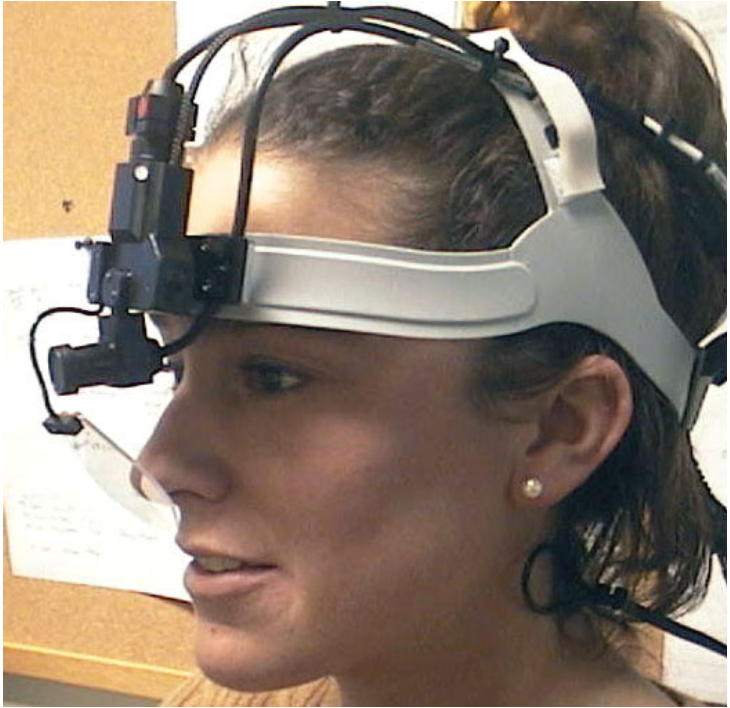
\includegraphics[width=0.75\linewidth]{images/headmounted_goldberg2002eye.png}
    \caption{
        Example of a head-mounted eye tracking device \autocite[12]{goldberg2002eye}
    }
    %for reference to this figure
    \label{figure:HeadMounted}
\end{figure}

\subsubsection{Infrared light -- bright and dark pupil}
While using a remote eye tracking device to record someone's eye movements, the camera most likely uses infrared light as an illuminator. Thus, the light hits the front of the eye which is also called the cornea and afterward the back, the retina. 
Moreover, the reason why the infrared light is used instead of any other light source is that it would distract the user while viewing the test material \autocite[]{poole2006eye, biedert2010eyebook}.

The two most known techniques, as mentioned by \textcite[]{goldberg2002eye}, are known as the bright and the dark pupil method. The bright pupil has the infrared placed in the same axis and ideally the same place as the camera. Therefore, the pupil is illuminated and brighter than the iris (this exact same effect leads to red eyes photos). The second method, dark pupil, has the illumination source placed on a different axis as the camera recording the eye. That leads to the pupils being darker (see Figure \ref{figure:DarkBright}). To gain improved results, these two methods can be used within the same eye tracking device \autocite[]{tobii2018dark, goldberg2002eye}. 

\begin{figure}[!ht]
    \centering
    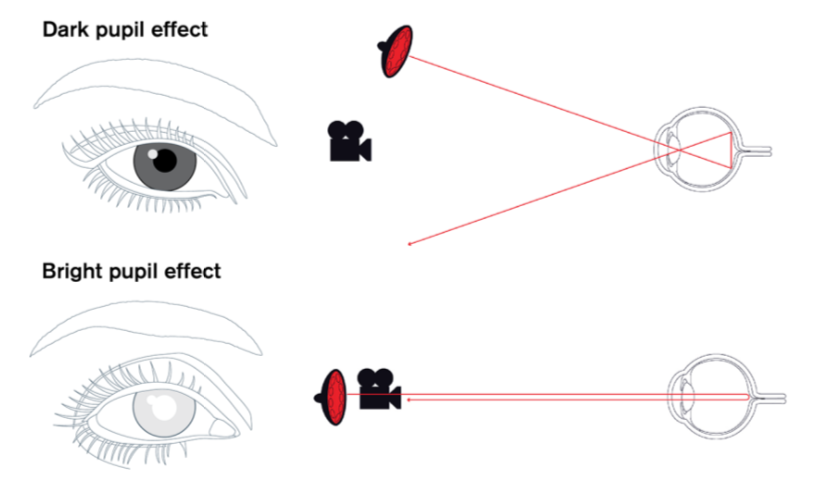
\includegraphics[width=1\linewidth]{images/DarkBright.png}
    \caption{
        Dark and Bright Pupil Method \autocite[]{tobii2018dark}
    }
    %for reference to this figure
    \label{figure:DarkBright}
\end{figure}


\subsection{Parameters}
\label{subsection:Parameters}
When an eye tracking device records a subject's eye movements, raw data can be collected. For instance, the most common element can be gaze points, which are points that get visually focused by the human's eye \autocite{bojko2009informative, vspakov2007visualization}. To extract valuable and applicable information out of the obtained raw data, \textcite[]{blascheck2014state}  suggests to aggregate it into fixations and saccades. 
Nowadays those are the two most commonly used parameters \autocite{bruneau2002eyes}. Thus, this section will provide a brief overview of the most essential and relevant parameters.

\subsubsection{Fixations}
A fixation is understood as a steady gaze at one point \autocite[]{buscher2009you}.  In the context of reading, as \textcite[]{beymer2007eye} annotate in their paper, fixations are moments where the gaze is paused on a word or a group of words. 
Normally a fixations duration lasts about 200-300 ms \autocite[]{kasneci2015online}. As stated by \textcite[]{buscher2009you}, to be considered a fixation the gaze must at least last 80-100 ms. Accordingly, during that time the brain can process the ingested information. Aside from that, a field where many foveal fixations take place is called an area of interest (AOI) \autocite[]{djamasbi2014eye}. For example, a webpage can be divided into different areas of interest (see Figure \ref{figure:AOI}).  On the one hand, when specific AOI's are used, one area can be simply a picture or the heading of a webpage. On the other hand, using broad AOI's, the page gets partitioned into larger parts like heading, pictures and text \autocite{djamasbi2014eye}. \\

\begin{figure*}[t]
    \centering
    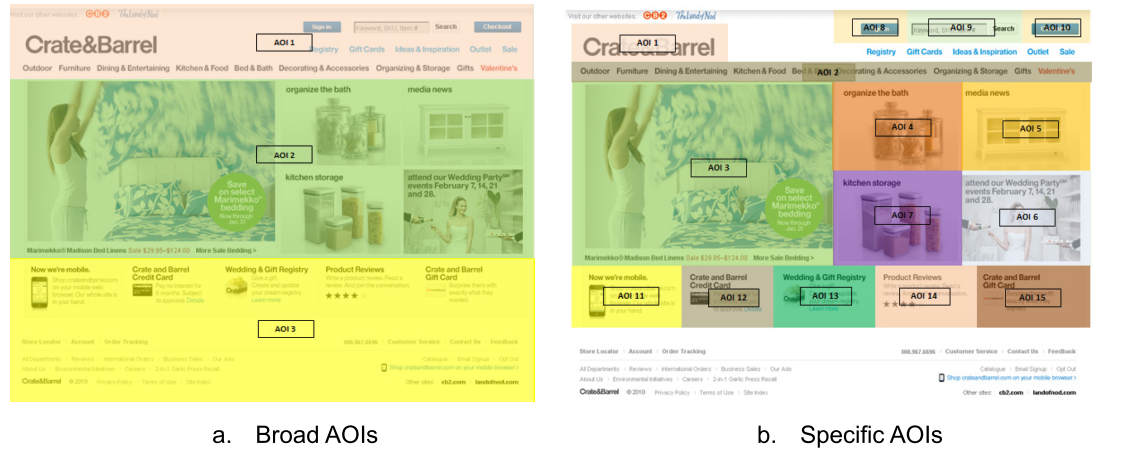
\includegraphics[width=0.75\linewidth]{images/AOI_djamasbi2014eye.png}
    \caption{
        Webpage divided into areas of interest (AOI) \autocite[48]{djamasbi2014eye}
    }
    %for reference to this figure
    \label{figure:AOI}
\end{figure*}

According to \textcite[]{grzyb2016eye}, when a user is looking at a website and an eye tracking device is set up, not all recorded fixations are detected correctly.
For instance \textcite[]{bruneau2002eyes} states in his paper, that not all eye movements seem to happen voluntarily. 
Despite the fact that fixations may not be an entirely flawless eye tracking parameter, \textcite[]{biedert2010eyebook} mention in their paper that information can only be correctly discovered with fixations.

\subsubsection{Saccades and Scanpaths}
Another significant parameter is the saccade which is the counterpart to fixations \autocite{goldberg2002eye}. They are short and fast movements between two points, the before mentioned fixations \autocite{goldberg2002eye, beymer2007eye}. Saccades are the quickest movements the body is able to achieve and typically last 30 to 80 ms \autocite[]{blascheck2014state}. \\
Furthermore, the scanpath is an important metric in terms of fixations and saccades. Scanpaths consist of alternating saccades and fixations. They reveal information about where the user looks first because scanpaths gives information in which order they look at what part of a website. Therefore, it can offer insights into a user's experience and additionally their behavior when they observe or interact with a website \autocite[]{lorigo2008eye, blascheck2014state}. Figure \ref{figure:Scanpath} shows scanpaths on a website, where the dots are the fixations and the lines are the saccades. \\
In the context of reading text on a website, a saccade is habitually a forward movement for around 8-12 characters in the text that is being read as \textcite[]{beymer2007eye} are explaining in their paper.

\begin{figure}[!ht]
    \centering
    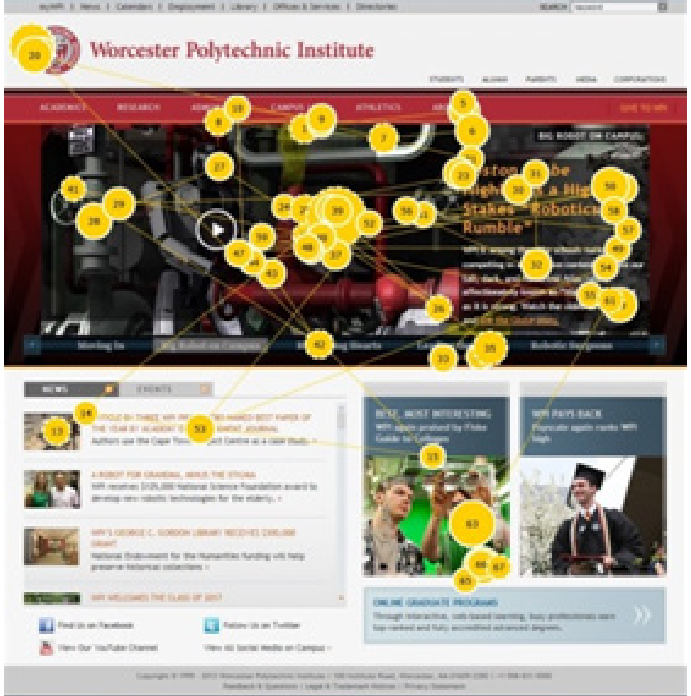
\includegraphics[width=1\linewidth]{images/scanpath_djamasbi2014eye.png}
    \caption{
       One possible way to visualize scanpaths \autocite[43]{djamasbi2014eye}
    }
    %for reference to this figure
    \label{figure:Scanpath}
\end{figure}

\subsubsection{Regressions}
Saccades are usually only forward movements, hence fast backward movements are called regressions \autocite[]{reichle1998toward}. 
\textcite[]{rayner1998eye} claims in his paper that regressions add up to 10 - 15 \% of the before mentioned saccades.
While reading a passage of a text, regressions are movements to the left of the line, mostly a few characters back, sometimes earlier words or occasionally even a whole sentence. Therefore \textcite[]{kruger2014subtitles} suggest in their paper that this could be an indicator of having troubles in processing the reading material or merely just oculomotor errors. Although most of the times the reader is not aware of those movements \autocite[]{reichle2003ez, biedert2010eyebook}.

\subsubsection{Pupil size}
As \textcite{goldberg2002eye} is describing in their paper one of the main reasons why someone's pupil size may change is increasing or decreasing illumination. For example, an eye tracking study can include videos or something else that is presented to the subject. If that happens, brightness may change very often in the shown material. As a consequence, the pupil size is constantly altering. To reestablish a more constant pupil size, the brightness of the room can be adjusted \autocite[]{goldberg2002eye}.
For example, the eye's pupil dilation can reveal whether the user finds interest in the website the look at or not. Hence, when the pupil is bigger, the user is also more interested as well as aroused, and when the pupil is smaller, the user does not find much interest in the material \autocite[]{joachims2017accurately}.\\
It is disputed that pupil dilation as a parameter can be an unreliable source because not only the text, but every little detail goes into one's reading experience. For example, sudden sounds in the surrounding area can play a part in one's change of pupil size when reading a text. 
Despite that, pupil dilation in a controlled environment, regarding time and space, can still say a lot about a user's experience on a website \autocite[]{bruneau2002eyes}.

\subsection{Results and Visualization}
\label{subsection:ResultsVisualization}
Once the eye movements of a person got recorded, the raw eye tracking data can be further processed. There are different methods to visualize the various eye tracking parameters. This following section will address today's most commonly used techniques and try to gauge which one is the most efficient.

\subsubsection{Statistical visualization approach}
The first approach for visualizing data are commonly used methods from statistics that are likewise used in eye tracking \autocite{blascheck2014state}. Raw eye tracking is primarily nothing more than mathematical or cartesian coordinates \autocite{blascheck2014state, biedert2010eyebook}. In addition to that, the raw data can contain information about the position of a user's head \autocite[]{biedert2010eyebook}. 
As \textcite[]{blascheck2014state} states in their paper, these statistical approaches are not exclusively constructed for eye tracking data. There are the three following alternatives to visualize the data: line chart, bar chart and scatter plot. The first one is the line chart which mostly displays mini-movements, slides, saccades or the mean time of fixations. The second is a bar chart which is typically used in the form of a histogram where the mean fixation duration is portrayed. And the third and last one is called a scatter plot which often illustrates saccadic movements \autocite[]{blascheck2014state}.
As mentioned before, these three graphs are not explicitly made to visualize eye-tracking data, therefore they may not be the best option to visualize these specific results.  Although all three graphs (see Figure \ref{figure:Statistics}) represent the same set of data, eye tracking data can be represented in many different ways and may mislead. 

\begin{figure}[!ht]
    \centering
    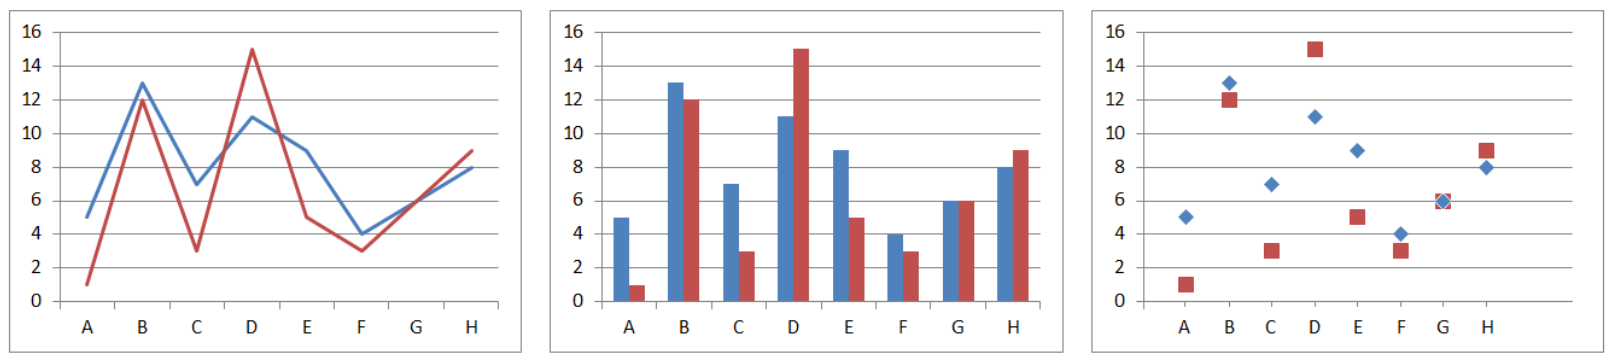
\includegraphics[width=1\linewidth]{images/statistics_blascheck2014state.png}
    \caption{
       Statistical representation of eye tracking data \autocite[7]{blascheck2014state}
    }
    %for reference to this figure
    \label{figure:Statistics}
\end{figure}


\subsubsection{Heat maps}
When it comes to visualizing the results of the gathered eye tracking data, one of the most common methods are heat maps. \textcite{bojko2009informative} state in their paper that one of the reasons why heat maps are often used is that they are simple to produce. 
A heat map can illustrate the number of fixations by coloring the most looked at points and parts of a website in a two-dimensional graph. Therefore, heat maps receive their name from the colors, which correspond to temperature. For example, red and yellow on the heat map portray the most frequently looked at points \autocite[]{bojko2009informative}. 

As \textcite[]{bojko2009informative} explains in their paper, heat maps are not a solution for every task that is being recorded with an eye tracking device. 
For example, when heat maps are being used to test if an element is poorly placed on a website. To get more realistic and reliable results, it would be necessary to put the desired item in more than one areas of the website and then repeat the trial. However, this would lead to a comparison between the accumulated data and its heat map, which is also not a reliable source to interpret a user's behavior \autocite[]{bojko2009informative}. 
In addition, according to the study of \textcite[]{djamasbi2010efficiency}, comparing two heat maps is not possible because they are not standardized in the sense of fixation quantity. Although both heat maps illustrate the fixations that were recorded before, the number of the fixations may differ. Therefore, two comparable heat maps must have the same amount of fixations to provide relevant results \autocite[]{djamasbi2010efficiency}. 

Furthermore, heat maps are not always an excellent representation of eye tracking data, because the colors are very opaque so that the original picture on the screen is not clearly visible anymore. To minimize this problem in a lot of studies the heat maps are turned into shadow maps where the image behind the overlapped map is still detectable \autocite[]{vspakov2007visualization}. Another alternative to avoid the opaqueness of heat maps are focus maps, where the important and more looked at points are visible and the rest of the picture is black \autocite{kruger2014subtitles}.

\subsubsection{Area of interest map}
An area of interest is a part of a website where plenty of fixations are recorded. To visualize and group them in the best way possible, a website can be divided into regions or areas of interest. These regions are either specific (e.g., items like buttons, pictures, ads) or rather global (e.g., top, middle, bottom of a webpage) \autocite[]{gonzalez2011different, djamasbi2014eye}. To gain more information about a website and how a user views it a fixation map and the areas of interest are combined. This resulting map provides a lot of information, for example, whether or not a specific part of a website is exciting. Furthermore, with the help of fixation timing, an AOI map can give information about the order in which the user views a webpage \autocite[]{djamasbi2014eye}.

\subsubsection{Gaze plot}
A third approach to visualizing eye-tracking data is using gaze plots. Similar to the already mentioned heat maps and attention maps gaze plots also use information about a user's fixation \autocite[]{kurzhals2016gaze}. \textcite[]{kurzhals2016gaze} also mentions that gaze-points not only display fixations but also take scanpaths, alternating fixations and saccades, into account. 

\selectlanguage{english}
\begin{quote}
``The spots on the gaze plot represent fixations, with larger spots representing longer fixations. The numbers in the spots represent the order of fixations and the lines indicate saccades.''
\autocite[]{djamasbi2014eye}
\end{quote}

As a consequence, similar to heat maps, gaze plots have dots all over the place, and the whole view is clustered with them. Therefore, the picture with all its items behind is not clearly visible anymore as \textcite[]{djamasbi2014eye} indicates in their paper.

\subsubsection{Gaze stripes}
And lastly, there is another method that is called gazed stripes and is imaged-based.

\selectlanguage{english}
\begin{quote}
``The visualization with gaze stripes for multiple participants is based on two data sources: the visual stimulus that was investigated by the participants and the spatio-temporal point-based gaze information that was recorded by an eye tracker.''
\autocite[3]{kurzhals2016gaze}
\end{quote}

\textcite[]{kurzhals2016gaze} introduce a new kind of visualization method. This method does not require pre-defined areas of interest because it uses the image around the gaze point. The method will work for static as well as dynamic sensory input. Furthermore, it will make it more accessible to interpret scanpaths. 
However, this method brings one issue along. For example, if the used stimuli contain similar colors, it becomes hard to differentiate between the separate objects in the picture \autocite[]{kurzhals2016gaze}.

%SEARCH ENGINE - SEARCH ENGINE - SEARCH ENGINE - SEARCH ENGINE - SEARCH ENGINE - SEARCH ENGINE
\section{Application Case - Search Engine (Search Engine Result Pages)}
\label{section:SearchEngine}
This following chapter will discuss the previously collected knowledge concerning information processing and eye tracking. Furthermore, search engines and the associated result pages will be taken into account as one of many possible application cases when it comes using eye tracking as a research method.
\subsection{Information Processing and SERP}
\label{subsection:ReadingSERP}
When it comes to search engines, there has been done a lot of research to optimize the presentation of the results that are shown on the result page.  In order to enhance the user's experience, display the most appropriate and relevant links at the top, and adjust the SERP as good as possible, it is essential to understand how the user observes the result page \autocite{buscher2010good, liu2015influence}.
For the longest time, displaying webpages as the results is a search engine's most important purpose. Besides, a search engine also presents advertisements, maps, images, videos, news and more results on their search engine result page. Nowadays, when mainly considering the links to webpages and their corresponding abstracts, which is the first page a user sees after entering a query and also the main result page of the search engine, a SERP is essentially built the same way as seen in Figure \ref{figure:ModernSerp}.
The result page contains elements like the search bar and button, advertisements with links and abstracts, fundamental links to webpages that match the search query, pictures and links to videos \autocite{wang2016beyond}.

\begin{figure}[!ht]
    \centering
    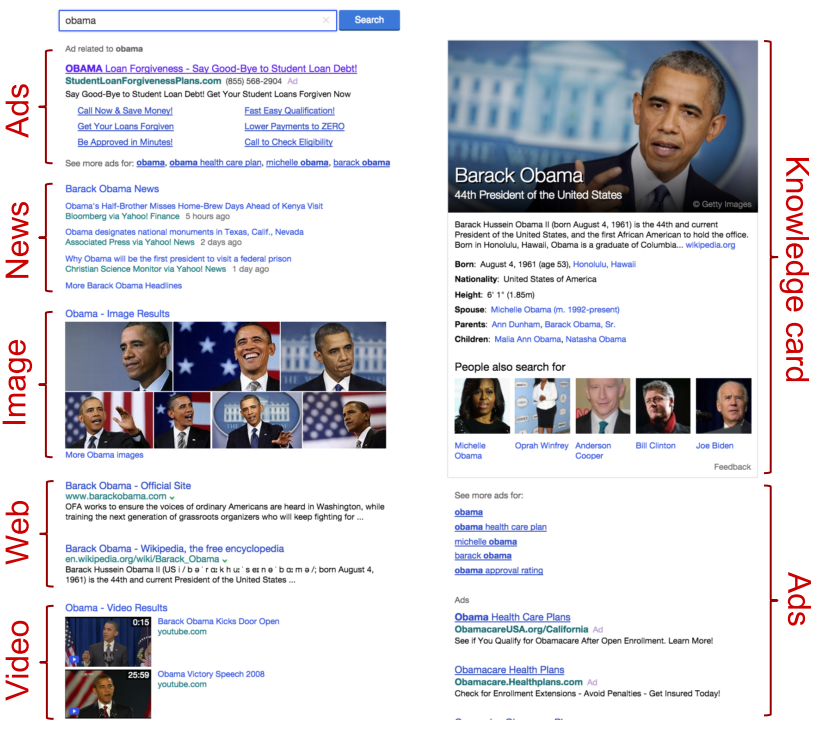
\includegraphics[width=1\linewidth]{images/SERP_wang2016beyond.png}
    \caption{
        Example of a modern Search Engine Result Page \autocite[104]{wang2016beyond}.
    }
    %for reference to this figure
    \label{figure:ModernSerp}
\end{figure}

As \textcite{lewandowski2015evaluating} is explaining in their paper, a few years ago SERPs were structured differently. For instance, the search engine result pages were built after the "ten blue links"-principle. Hence, those pages generally just consisted of the essential ten links to webpages. Moreover, this principle indicates and reinforces the user's behavior to only look at first few results that a search engine computes \autocite{lewandowski2015evaluating, liu2015influence, wang2016beyond}. Another way to describe this convention is called "organic results". Accordingly, see Figure \ref{figure:OrganicResults}, there is a section with the "organic results" on a SERP with no advertisements presented and solely the results and their abstracts get displayed \autocite{buscher2010good}.

\begin{figure}[!ht]
    \centering
    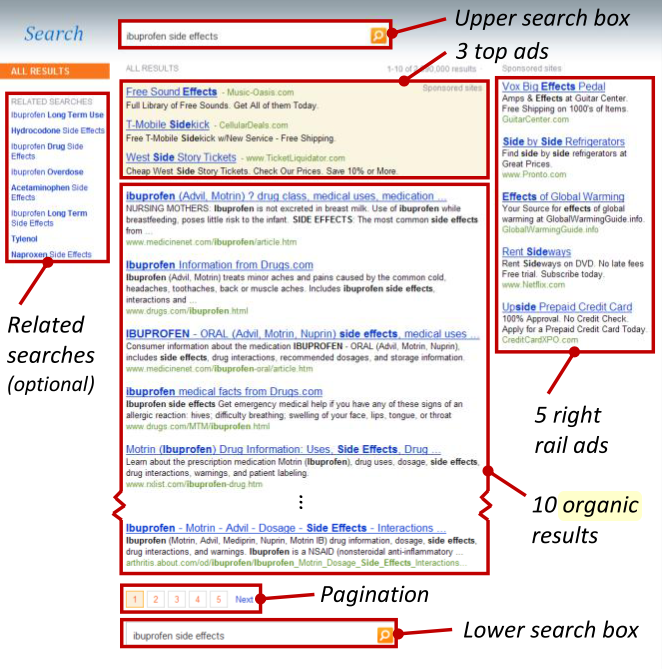
\includegraphics[width=1 \linewidth]{images/organic_buscher2010good.png}
    \caption{
        Example of the "ten blue links" or "organic results" on a modern SERP \autocite[3]{buscher2010good}
    }
    %for reference to this figure
    \label{figure:OrganicResults}
\end{figure}

On a result page that is built after the "ten blue links"-principle the result-links are ranked based on relevance. Therefore, the search engine makes estimations and evaluations itself, whether the user would find the shown results fitting or not. This process is also called the "probability ranking principle" \autocite{wang2016beyond}. This policy is reasonably justified because the user usually never looks further than the first suggested page out of the various recommended pages as \textcite{lewandowski2015evaluating} is explaining in their paper.
One of the most prominent parts of the website is the section that includes pictures. Furthermore, the human eye tends to pay increased attention to images in comparison to plain text. When an eye tracking device is being used to record the user's eyes,  images get looked at more. This phenomenon is called the attention bias, more specifically the vertical bias.
The same exact issue seems to appear with the before mentioned "ten blue links" that are summed up into a vertical result \autocite{wang2016beyond}.
In contrast, \textcite{liu2015influence} explains in their paper that not all pictures get the same amount of attention. In their study, they found that images that happen to be a part of a preview of news content get overlooked most of the times. Only images that are not directly attached to any kind of article or link get more attention \autocite{liu2015influence}.

\subsection{Different Search Engines -- different methods?}
\label{subsection:SearchEngine}
As \textcite{pan2007google, agrawal2015study} mention in their paper Google, Bing and Yahoo! are currently the most known and also most used search engines. Therefore this following section will look further into specific search engines, especially their methods and tools to present the best search engine result pages.

\subsubsection{Google, Yahoo!, Bing}
Google is by far the most used search engine, as \textcite{pan2007google} points out in their paper. The search engine receives more than 250 million queries a day and presents the appropriate results in the form of 25 billion web pages. In their article, they point out that people, but students primarily, tend to click on links and abstracts that are higher ranked, even though they are less relevant than the lower ranked ones. As a consequence, Google has the potential to influence our current society by presenting any kind of results and manipulate our way of information retrieval. During their study, they also found out, that Google works with the "ten blue links"-principle \autocite{pan2007google}.

\subsubsection{Other search engines}

\subsubsection{Comparison}

\section{Discussion}
\label{section:Discussion}
Discussion

\section{Conclusion}
\label{section:Conclusion}
Conclusion



 % the main text

%\input{acknowledgements}

%\ifmmtpaper\else % only use the following for thesis format

\newpage
\onecolumn    
\ifmmtlanguagegerman
\section*{Abkürzungsverzeichnis}
\else
\section*{Abbreviations}
\fi

\begin{table}[h]		
	\begin{tabular}{ll}
	    AOI & Area of interest \\
		SERP & Search Engine Result Page \\
		UX & user experience \\
	\end{tabular}
\end{table}

\listoffigures
\lstlistoflistings
\listoftables

\newpage

%\fi

\printbibliography

 % group open
\ifmmtpaper 
\begingroup 
    % is required because paper template messes with sizes
    \fontsize{12}{18}\selectfont        
    \setlength{\parindent}{0pt}
    \setlength{\parskip}{5pt plus 2pt minus 1pt}
    \sectionfont{\fontsize{14}{15}\selectfont}
\fi

\newpage
\onecolumn
\appendix

\textbf{\color{red} Anhänge löschen, die nicht verwendet werden.}

\section*{Appendix}
\addcontentsline{toc}{section}{Appendices}
\renewcommand{\thesubsection}{\Alph{subsection}}

\subsection{git-Repository}

Das Repository dient zur Dokumentation und Nachvollziehbarkeit der Arbeitsschritte. Stellen Sie sicher, dass der/die BetreuerIn Zugriff auf das Repository hat. Stellen im Sinne des Datenschutzes sicher, dass das Repository nicht für andere zugänglich ist.

Daten für Bachelorarbeit 1 und 2:

\begin{itemize}
	\item LaTeX-Code der finalen Version der Arbeit
	\item alle Publikationen, die als pdf verfügbar sind.
	\item alle Webseiten als pdf
\end{itemize}

Daten für Bachelorarbeit 2:
\begin{itemize}
	\item Quellcode für praktischen Teil
	\item Vorlagen für Studienmaterial (Fragebögen, Einverständniserklärung, ...)	
	\item eingescanntes, ausgefülltes Studienmaterial (Fragebögen, Einverständniserklärung, ...)
	\item Rohdaten und aufbereitete Daten der Evaluierungen (Log-Daten, Tabellen, Graphen, Scripts, ...)	
\end{itemize}

Link zum Repository auf dem MMT-git-Server {\url{gitlab.mediacube.at}}:

{\color{red}\url{https://gitlab.mediacube.at/fhs39868/Bachelorarbeit1_Isabella_Sperr}}

\subsection{Archivierte Webseiten}
% \show\UrlBreaks

\url{http://web.archive.org/web/20160526143921/http://www.gamedev.net/page/resources/_/technical/game-programming/understanding-component-entity-systems-r3013}, letzter Zugriff 1.1.2016

\url{http://web.archive.org/web/20160526144551/http://scottbilas.com/files/2002/gdc_san_jose/game_objects_slides_with_notes.pdf}, letzter Zugriff 1.1.2016




% group closing
\ifmmtpaper
\endgroup
\fi


\end{document}
